\documentclass{article}
\usepackage[a4paper, total={180mm, 260mm}]{geometry}
\usepackage{graphicx}
\usepackage{url}
\usepackage{natbib}
\usepackage{todonotes}
\usepackage{booktabs}
\usepackage{lineno}
\usepackage{color}
%\usepackage{auto-pst-pdf}
\usepackage[colaction]{multicol}
\usepackage{caption}
\usepackage{svg}
\usepackage{authblk}
\usepackage{standalone}

\usepackage[section]{placeins}


\linespread{1.5}

\makeatletter
\renewcommand{\maketitle}{\bgroup\setlength{\parindent}{0pt}
	\begin{flushleft}

		{\huge\textbf{\@title}}

		\bigskip

 		{\large\textbf{\@author}}

 		\bigskip

 		{\large{Draft current \@date}}

	\end{flushleft}\egroup
}
\makeatother

\newcommand{\multicollinenumbers}{
	\linenumbers
	\def\makeLineNumber{\docolaction
		{\makeLineNumberLeft}
		{}
		{\makeLineNumberRight}
		}
}

\newenvironment{figurehere}
	{\def\@captype{figure}}
	{}

% Title
\title{A Topic Model of Climate Change Literature}
\title{Words, words, words: Mapping the Matter of Climate Change Literature}
\title{A Topography of Climate Change Research}
\author[1,2]{Max Callaghan}

\affil[1]{Mercator Research Institute on Global Commons and Climate Change, Torgauer Straße, 10829 Berlin, Germany}
\affil[2]{School of Earth and Environment, University of Leeds, Leeds LS2 9JT, United Kingdom}

\begin{document}
\maketitle


\begin{linenumbers}

\noindent\textbf{\documentclass{article}

\begin{document}
	The massive expansion of scientific literature on climate change challenges the Intergovenmental Panel on Climate Change (IPCC)'s ability to assess the science according to its objectives.
	Moreover, the number and variety of papers hinders researchers of the science-policy interface from making objective judgements about those IPCC assessments. In this paper, we present a novel application of a machine-reading approach to model the topical content of papers on climate change. This dynamic topic model provides the basis for a \textit{topography} of climate change literature. The thematic development of the field is outlined and used to inform an analysis of the topics which are better and less well covered by IPCC reports.
\end{document}}



\bigskip

\noindent We live in an age of ``Big Literature'' 
\cite{Nunez-Mir2016}, where the science of climate change is expanding rapidly \cite{Grieneisen2011, Haunschild2016}. In the five years since the publication of the last IPCC assessment report \cite{IPCC2014c}, 201,606 papers were published (see Table \ref{tab}). This is almost as much as the 204,585 papers published during the first five assessment periods, a period of nearly 30 years. The vocabulary of the literature has also expanded - from 2,000 unique words in AR1 to 94,746 words so far in AR6 - indicating that the field has incorporated new content. For example, the zika virus, which was mentioned in 182 articles from 2014-2018, had never before been discussed in the titles or abstracts of articles relating to climate change. Yet it has emerged as a topic of high relevance: the incidence of the virus, the outbreak of which in Brazil in 2016 was declared a public health emergency by the WHO, is set to increase under rising global temperatures \cite{Rao2019}. Similar rapid emergences can be seen for [Intended] Nationally Determined Contributions ([I]NDCs) and Sustainable Development Goals (SDGs) in AR6, and Biochar and REDD (The United Nations Collaborative Programme on Reducing Emissions from Deforestation and Forest Degradation in Developing Countries) in AR5, among others. This large and rapidly evolving literature demands innovative machine-reading methods to enable understanding of the field at scale.


\begin{table}[htp]
	{\scriptsize
		\begin{tabular}{|l |p{1.8cm} p{1.8cm} p{1.8cm} p{1.8cm} p{1.8cm} p{1.8cm}|} 
\hline 
&\textbf{AR1} & \textbf{AR2} & \textbf{AR3} & \textbf{AR4} & \textbf{AR5} & \textbf{AR6}\\ \hline}
	\caption{Growth of Literature on Climate Change. A glossary of acronyms is provided in SI}
	\label{tab}
\end{table}


Research synthesis offers structured methodologies for integrating knowledge from bodies of evidence \cite{Chalmers2002}. Systematic reviews, which are common in the health sciences, collect all literature relevant to a specific question, in order to establish whether findings are consistent and generalisable \cite{Mulrow597}. Already in 1994, systematic review was being proposed as an answer to the ``small mountain of information'' presented by two million annual publications in biomedical literature \cite{Mulrow597}. Although climate change faces a similar scale problem, systematic review is little used in the field \cite{Berrang-Ford2015}. Systematic maps are a more recent methodological development, which show the state of the evidence in a broad subject area \cite{James2016}. There have been high profile calls to broaden the applications of evidence mapping in sustainable development \cite{McKinnon2015}, and they are similar underused in climate change, with only 25 of the more than 400,000 relevant papers containing the phrase "systematic map" in the abstract or title. 


In the research synthesis field, researchers are introducing new methods from natural language processing and machine-learning to scale up synthesis work \cite{OMara-Eves2015, Westgate2018a}. In the same way, this study uses topic modelling \cite{Blei2010} to map out the vast body of evidence on climate change. Topic modelling is an unsupervised machine-learning technique, where patterns of word co-occurrences in documents are used to learn a set of topics which can be used to describe the corpus. The word topic derives from the Greek word for place (topos), and by \textit{situating} the documents in a reduced-form projection of their thematic content (see Figure \ref{oecd_topic_map}), we create a \textit{topographic map} of the literature on climate change. Such a systematic engagement with the thematic content of the climate science is missing from the literature so far.%To our knowledge, this is the first 

Systematic maps can have several uses: from the identification of knowledge gaps and gluts to the can identification of authors or institutions with expertise on a subject. The map in this paper also has several potential uses, but we focus here on using the map to understand the evolution of relationship between the five IPCC assessment reports and the wider literature on climate change. Big Literature in climate change poses a great challenge to the IPCC, who's mandate is to comprehensively assess the science of climate change \cite{IPCC2013}. The ratio of studies cited in IPCC reports to the number or relevant studies has declined from 60\% to 20\%  \cite{Minx2017l}, thus increasing the risk of a lack of comprehensiveness, or even bias.  

What gets included in IPCC reports is also much discussed. Policymakers demand more solution-oriented knowledge \cite{Kowarsch2017}, and there have been calls for the inclusion of more knowledge from the social sciences \cite{Victor2015}. But what we say about the literature cited in the IPCC has often been limited by a failure to consider the context of the wider literature. 
A scientometric study from 2011 claimed that the IPCC gave a greater \textit{emphasis} to natural sciences and, within the social sciences, to economics \cite{Bjurström2011}. This claim has subsequently been interpreted as a disciplinary bias by the IPCC \cite{Hulme2010, Corbera2016} towards the natural sciences, but the study operationalised disciplinary emphasis as simply the share of citations from each field, and was based on analysis of the Third Assessment report, published in 2001. In the following sections, we compare distributions of literature in the subset that is cited by the IPCC and the wider corpora, to analyse the \textit{representation}, proportional or otherwise, of scientific fields, as well as of topics.

\subsection*{Proportionality in IPCC citations}


Figure \ref{oecd_rep}.a shows that the social sciences were indeed under-represented in the third assessment report, but by the fifth assessment report were over-represented. Likewise, other social sciences than economics have become better represented since AR3  (see figure \ref{subfield}f) with social \& economic geography (4.3\% of the literature), political science (1.0\%), and sociology (0.8\%) showing improved representation in AR5 compared to AR3, and Social and economic geography, political science, and other social sciences better represented than economics when taking into account the distribution of studies in the literature. 

This challenges what we think we know about the IPCC. The social sciences, by now, are actually the best represented field, with a share in the literature cited by IPCC reports [1.5] times as high as in the literature at large.  On the other hand the Agricultural Sciences and Engineering \& Technology have been consistently under-represented, with [2.5] and [3.5] times the share of studies in the wider literature than in the literature cited by the IPCC in AR5 respectively. % (Humanities are also underrepresented, but making up only 0.9\% of the wider literature, the proportionality is particularly sensitive).

\begin{figure}[htp]
	\begin{center}
		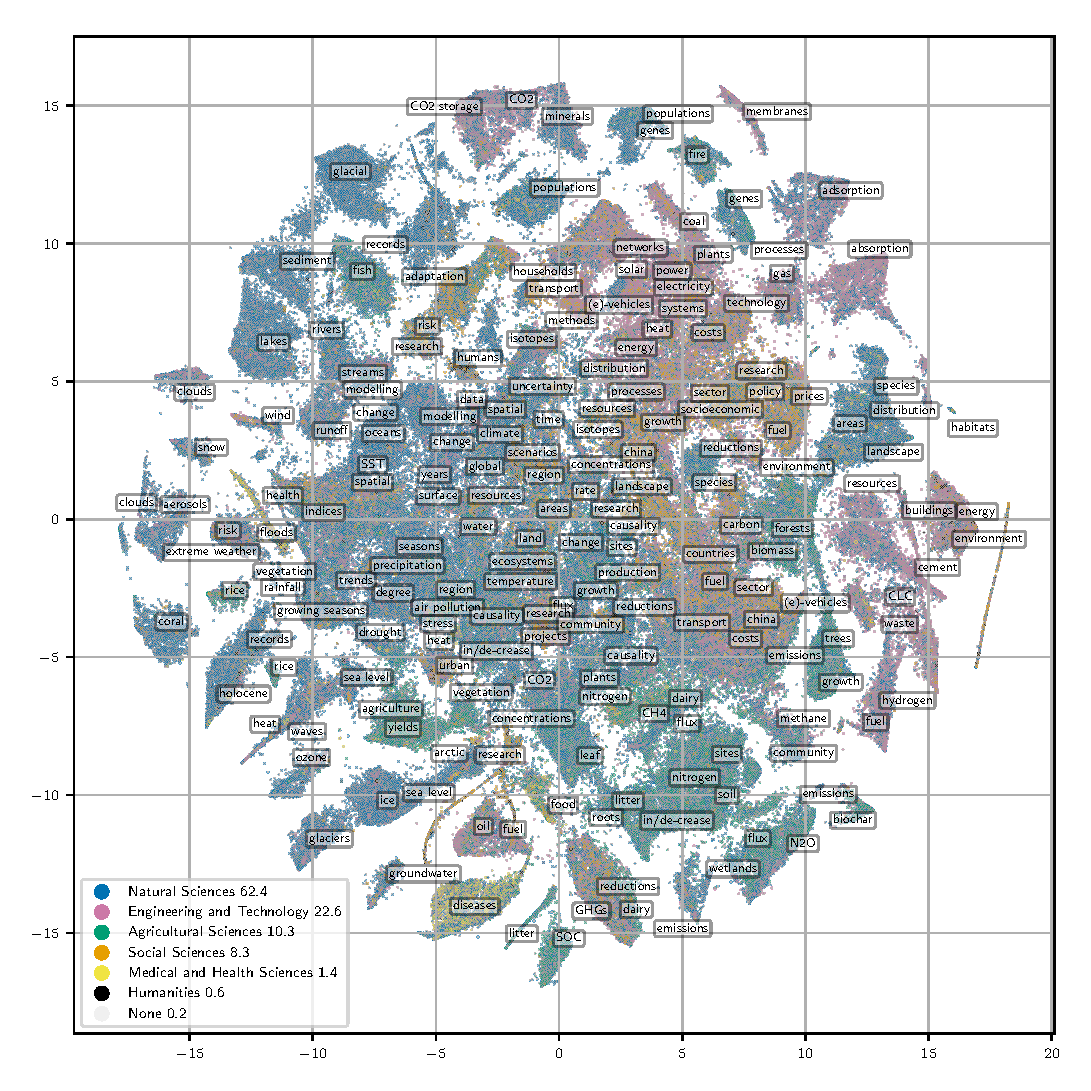
\includegraphics[width=180mm]{plots_pub/all_topic_words_oecds.png}
		\caption{A map of the literature on climate change. Document positions are obtained by reducing the topic scores to two dimensions via t-SNE Documents are coloured by web of science discipline category. Topic labels are placed in the center of each of the large clusters of documents associated with each topic. }
		\label{oecd_topic_map}
	\end{center}
\end{figure}


%\subsection*{A Topography of Climate Change Research}

Figure \ref{oecd_topic_map} shows the 400,000 documents on climate change in our dataset in a dimensionality reduction enabled representation of their topic structure, with topic labels placed near clusters of documents highly relevant to each topic. The map shows the high proportion of the natural sciences in climate change research, and the large proportion of the topic space dominated by natural science publications. These two features of the landscape account for the proportionally high share of natural science publications in IPCC citations.

The thematic structure of the literature also maps well to the disciplinary structure, with clusters of social science topics, such as \textbf{policy}, \textbf{research}, \textbf{sector} and \textbf{growth} in the centre right of the graph, and natural sciences on the left. With reference to figure \ref{dis-entropy}, we can identify the topics which are more or less distributed across disciplines. \textbf{Coral}, for example, is almost exclusively discussed in the natural sciences, while papers on socio-economic issues are discussed in a variety of disciplines. Further, by using the topographical map, we can dig down further into the subject matter that is more or less proportionately represented, within and across disciplines.






\begin{figure}[htp]
	\begin{center}
		\includegraphics[width=180mm]{plots_pub/big_panel_representation.pdf}
		\caption{Representation in IPCC reports: \textbf{a)} by discipline, \textbf{b)} by social science proportion of WG 3 topics, \textbf{c)} and novelty of all topics, where topics in the highest and lowest 10\% of either axis are labelled. Topics are coloured according to the working group from which they receive the most citations. Representation is the share of the subset of documents being cited by the IPCC divided by the share of the subset in the whole literature. The log is taken so that 0 is equal to perfectly proportional representation, and -1 and 1 are equally under and over represented.}
		\label{oecd_rep}
	\end{center}
\end{figure}

 %, and to further investigate the content of the documents that are more less proportionately represented in the IPCC.


\begin{figure}
	\begin{center}
		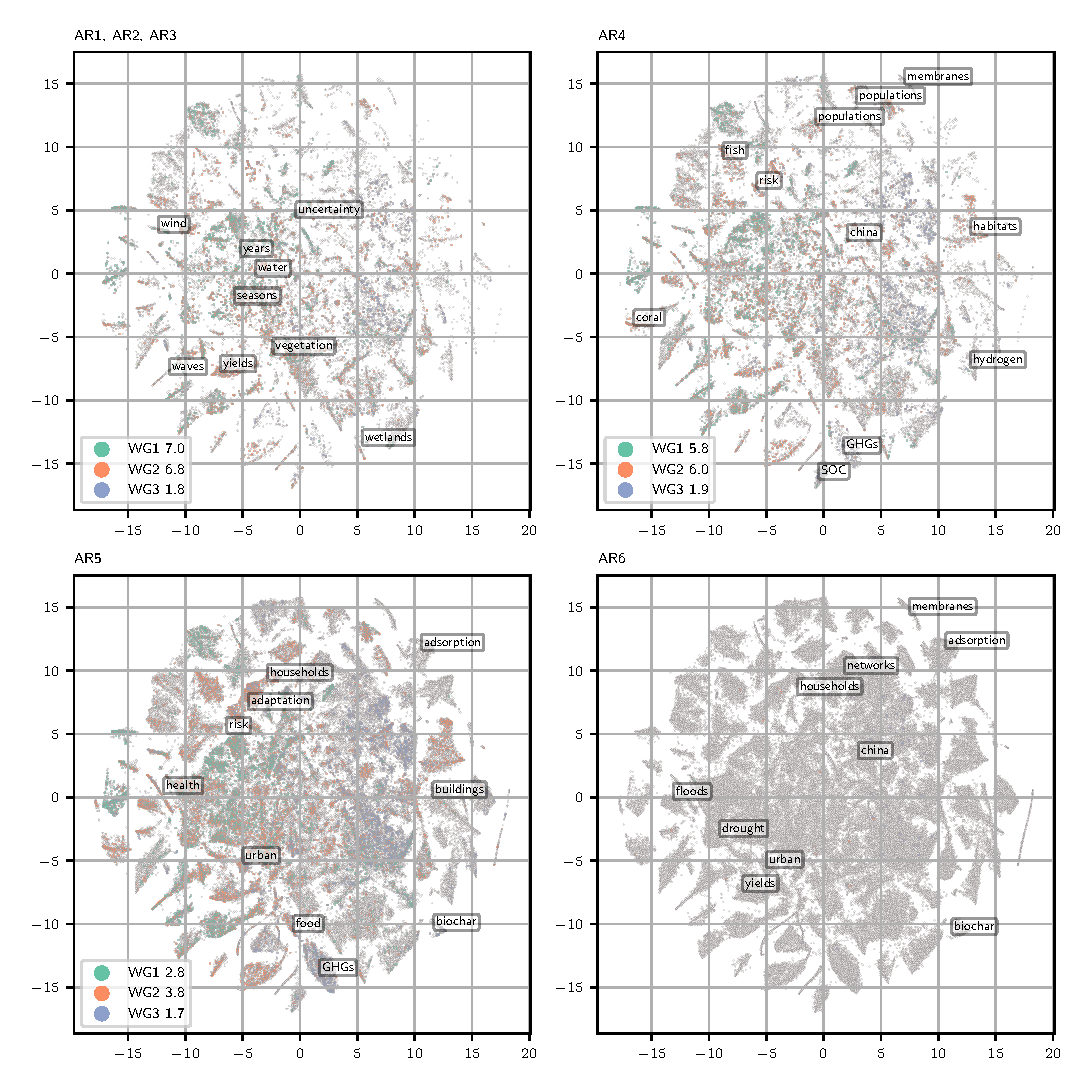
\includegraphics[width=180mm]{plots_pub/topic_evolution_4.png}
		\caption{Evolution of the landscape of climate change literature}
		\label{evolution-map}
	\end{center}
\end{figure}

\subsection*{Supply and demand for solutions-oriented knowledge}

Figures \ref{oecd_rep}b and \ref{oecd_rep}c plot the representation of the topics shown in the map. Figure \ref{oecd_rep}c shows that topics more commonly cited by IPCC working group I are older and largely better represented in IPCC reports. It makes intuitive sense that these topics, for example \textbf{ozone}, \textbf{oceans}, \textbf{clouds}, \textbf{aerosols} and \textbf{sea levels}, are older, predominantly cited by WG I, and well cited by IPCC reports, as these are some of the core topics of the physical science of climate change.

The topics in the lower right of the graph are the most pertinent to the question of whether the IPCC is well representing knowledge on climate change. These topics are newer and until now have been under-represented in IPCC reports. They are the topics that could be seen as potential gaps in the IPCC's coverage of the science. Because they are new areas of knowledge, they may be highly salient in a periodic assessment process. These topics are primarily in working group III (mitigation), with the exception of adsorption, CLC and hydrogen which are primarily of relevance to WG III but are miscategorised due to the low number of citations of relevant documents and citations of tangentially relevant documents by other working groups \footnote{For example, the word ``capacity" is relevant to the adsorption topic, so documents talking about adaptive capacity receive a low relevance score for that topic. Because only very few documents highly relevant to the adsorption topic (in that they talk about adsorption or adsorptive capacity) are cited by the IPCC, and many of the weakly relevant documents are cited by the IPCC, the sum of the topic scores of the weakly relevant WG II documents outweighs the sum of the topic scores of the strongly relevant WG III documents}.

Although it is perhaps not surprising that these newer topics are less well represented than the older topics that make up the core of the physical science research on climate change, the difference between these new topics and other new topics that are better represented is intriguing. This difference is visible in figure \ref{evolution-map}, where the fastest growing topics in each period are labelled, and the documents are coloured according to the working group, if any, which cites them. In AR5, the clusters of documents around the \textbf{adsorption}, \textbf{buildings}, and \textbf{biochar} topics contain few IPCC citations, whereas the clusters around \textbf{food}, \textbf{health}, \textbf{adaptation}, and \textbf{GHGs} contain more. This is also evident in figure \ref{oecd_rep}c, where these topics display corresponding representation values. The IPCC, then, has been better at integrating new knowledge from these topics, and in general better at integrating new knowledge from WG II  than WG III topics.

Within WG III topics, those that are well represented contain a greater proportion of social science research (figure \ref{oecd_rep}b). The topics \textbf{countries}, \textbf{policy}, and \textbf{prices} are close to a proportional representation and are made up of around 30\% social science research. \textbf{Waste}, \textbf{biochar}, \textbf{cement} and \textbf{coal}, are more than 3 times more prevalent in the wider literature than in the literature cited by the IPCC, and are made up of around 5\% social science research. This pattern is not visible in other working groups (see Figure \ref{socsci-wgs}), and complicates the perception of the under-representation of the social sciences.


Recalling policymakers' demands for more solution-oriented assessments \cite{Kowarsch2017}, we could also interpret the topics that are newer and under-represented as ``solutions-relevant''. Many deal with negative emissions, or with mitigation (or to a lesser extent adaptation) options in the transport, buildings and power sectors. All are arguably related to climate solutions. However, while policymakers' demands for solutions-oriented knowledge were rather about policy options, these under-represented new topics deal with more technical solutions and are found rather in technical disciplines within engineering \& technology and the agricultural sciences.

\subsection*{The IPCC as an informed decision-maker on topical representation}

Deciding on the optimal proportion of each topic's literature to be cited by the IPCC is not a trivial task. A perfectly proportional representation of each topic is almost certainly not optimal, and as such, decisions about which topics to over-, or under- represent are best made by experts, not by a computer. Indeed, the IPCC itself is the best-placed institution to make these decisions. But in the age of ``Big Literature'' \cite{Nunez-Mir2016}, these decision should at best be underpinned by systematic knowledge of the landscape of the literature, and made in discussion with the wider research community, funders, policymakers and other stakeholders.

The analysis in this study provide a useful input to this discussion. It could be argued that the under-represented technical literature on specific technological or sectoral solutions is not relevant to policymakers, and that working group III should give more weight to evidence about general policy instruments such as carbon taxes. Conversely, one could argue that establishing a technical understanding of specific climate solutions is as important a task as establishing a technical understanding of the physical science of climate change. The desire for more social science research in IPCC reports may imply, given the evidence here, that more social science research on climate change needs to be produced and funded, rather than that the IPCC should cite more of what already exists. Or, one could argue that, in light of the evidence that there is little social science research on solutions-relevant, under-represented topics, that the social sciences could do more to address technical or specific solutions such as negative emissions, green concrete, or waste and recycling.

An understanding of the topography of the literature helps bring these arguments to the foreground, and allows them to be made in an informed way. Machine reading the literature in this way is not without its limitations though, and indeed many are apparent in this analysis. The corpus of potentially relevant literature is of course much wider than what is included in this study. The analysis excludes studies about climate change that do not match our query, studies relevant to tackling climate change that do not mention it specifically, studies written in languages other than English (unless the abstract has been translated), studies not indexed in the Web of Science, and reports published outside peer reviewed journals, not to mention Indigenous knowledge \cite{Ford2016b}. Despite this, unless the social science literature in the above categories is cited systematically less often  by the IPCC than the social science literature that was analysed in this study, then the main conclusions of this study hold. Topic models also carry limitations, and do not present the \textit{objective} truth about a corpus, given that they can be sensitive to modeller choices, such as the number of topics. However, the observations about the under-representation of solutions-relevant topics are robust across a broad range of topic numbers \ref{top-rep-ks}.

Computational methods then, provide \textit{assistance} to humans in understanding a climate change literature that is produced by human individuals and institutions.  As in other areas of machine learning \cite{Barocas2016}, computational assessments of the literature run the risk of reproducing biases or gaps in the training data. However, just as with other applications of machine learning, machine-reading the science of climate change can provide information that helps us to understand gaps in what we have knowledge about, and potential biases, or options for emphasis, in how we represent that knowledge in the IPCC. In this way, we can more effectively meet the challenges posed by Big Literature to global environmental assessments.
%Machine learning approaches to understanding scientific literature are already latently present in our engagement with  when we use academic search engines or are recommended articles 

\end{linenumbers}

\appendix

%\listoffigures
\linespread{1}
\bibliography{Mendeley}
\bibliographystyle{unsrt}

\documentclass{article}
\usepackage[a4paper, total={6in, 8in}]{geometry}
\usepackage{graphicx}
\usepackage{url}
\usepackage{natbib}
\usepackage{todonotes}
\usepackage{booktabs}
\usepackage{lineno}
\usepackage{color}
%\usepackage{auto-pst-pdf}
\usepackage[colaction]{multicol}
\usepackage{caption}
\usepackage{svg}
\usepackage{authblk}
\usepackage{standalone}
\usepackage[section]{placeins}

\makeatletter
\renewcommand{\maketitle}{\bgroup\setlength{\parindent}{0pt}
	\begin{flushleft}
		
		{\huge\textbf{\@title}}
		
		\bigskip
		
		{\large\textbf{\@author}}
		
		\bigskip
		
		{\large{Draft current \@date}}
		
	\end{flushleft}\egroup
}
\makeatother


\begin{document}
	% Title
	\title{A Topic Model of Climate Change Literature}
	\title{Words, words, words: Mapping the Matter of Climate Change Literature}
	\title{A Topography of Climate Change Research - Methods}
	\author[1,2]{Max Callaghan}
	
	\affil[1]{Mercator Research Institute on Global Commons and Climate Change, Torgauer Straße, 10829 Berlin, Germany}
	\affil[2]{School of Earth and Environment, University of Leeds, Leeds LS2 9JT, United Kingdom}
	\maketitle
	\begin{linenumbers}
	
	\setcounter{figure}{0}
	\renewcommand\thefigure{SI.\arabic{figure}}  
		
	\subsection*{Data}
	
	This study reproduces the query developed by \citep{Grieneisen2011}, which is carried out on the Web of Science core collection. Though not exhaustive, the Web of Science gives a good coverage of the literature in major peer-reviewed journals.	Each document is assigned to an assessment period according to the timeline shown in table 1.
	
	We use the references scraped from IPCC assessment reports from \citep{Minx2017l}, and attempt to match these with the results from the web of science. Table \todo{}[x] shows the percentage of IPCC citations matched in each working group for each assessment report.
		
	\subsection*{Pre-processing}
	
	Data quality in earlier Web of Science results is poorer, and some documents have missing abstracts. In the quantification of the size of the literature and its vocabulary in table [], titles are substituted for abstracts where they are not available.  The words of the documents are lemmatized/stemmed, replacing different forms of the same word (i.e. word/words) with a single instance. Commonly occuring words, or ``stopwords'' are removed, as are all words shorter than 3 characters, and all words containing only punctuation or numbers.
	
	The documents are transformed into a document-term matrix, where each row represents a document, and each column represents a unique word.  Each cell contains the number of that column's terms in that document. Only terms which occur more than once are considered.
	
	For the calculation of the topic model, documents with missing abstracts are ignored, and the document term matrix is transformed into a document
	frequency-inverse document frequency (tf-idf) matrix, where scores are scaled according to the frequency of their occurence in the corpus. This gives more weight to terms which appear in few documents, and less weight to those which appear in many.
	
	\begin{equation}
	tf(t,d) = f_{t,d} \mathrm{,}\quad idf(t,D) = \log\frac{N}{|\{d \in D:t \in d\}|}
	\end{equation} 
	
	\subsection*{Topic Model}
	
	We use non-negative Matrix Factorisation (NMF) \cite{Lee1999}, an approach to topic modelling which factorises the term-frequency-inverse document frequency matrix \( V \) into the matrices \(W\), the topic-term matrix, and \( H \) the document-topic matrix, whose product approximates \(V\):
	
	\begin{equation}
		V_{i\mu} \approx (WH)_{i\mu} = \sum_{a=1}^{r}W_{ia}H_{a\mu}
	\end{equation}
	
	As demonstrated in Figure \ref{doc-topic}, each topic is represented as a set of word scores, and each document a set of topic scores. The combination of the two give the word scores in the document. For clarity in the figure, these are shown as simple counts, but in the model these are scaled according to each term's frequency within the corpus as explained above.
	
	Topics are calculated using the scikitlearn library \cite{Pedregosa2011}, and are saved in a database and topic visualisation system based on \cite{Chaney2012} \footnote{The system adds new functionality to \cite{Chaney2012} and combines it with a system for managing sets of documents and queries. The code and additional information is published online at \url{https://github.com/mcallaghan/tmv}}. 	
	
	\subsubsection*{Model selection}
	
	Topic models are calculated for 70, 80, 90, 100, 110, 120, 130 and 140 topics. The relative usefulness of each model was assessed subjectively by the authors, based on inspection of the online visualisation tool, and the spreadsheet \textbf{topic\_comparison.xlsx} accompanying the supporting information. The spreadsheet shows each set of topics in adjacent columns. Topics from each model are placed next to the topics with the largest number of each topic's 10 highest scoring words in common. This helps authors to find an appropriate level of granularity for the analysis. 
			
	\subsubsection*{Topic Representation and Newness}
	
	To calculate topic representation in IPCC reports we divide each topic's share in the subsample of documents cited by IPCC reports by its share in the whole corpus. 
	
	We calculate a topic's total score as the sum of document-topic scores. A topic's window score is the sum of document-topic scores considering only documents in the given time window. To represent a topic's newness, we multiply each assessment period number by the share of it's total score occurring in that window, and take the mean of these scores. A topic in which 100\% of documents which make it up occurred in assessment period 1 (6) would thereby receive a score of 1 (6), while a topic evenly distributed across all assessment periods would receive a score of 3.5.
	
	
	\subsubsection*{Disciplinary Entropy}
	
	Disciplinary Entropy inverts the measurement of a conference's topical diversity suggested in \cite{Hall2008}, by measuring a topic \(z\)'s entropy \(H\), where 
	
	\begin{equation}
		H(f|z) = -\sum_{i=1}^K \hat{p}(f|z) \log \hat{p}(f|z) 
	\end{equation}
	
	based on the empirical distribution of a field \(f\) in the documents \(d\) in each topic:
	
	\begin{equation}
		\hat{p}(f|z) = \sum_{d:z_d=z} \hat{p} (f|d) \hat{p} (d|z)
	\end{equation}

	\begin{figure}
		\begin{center}
			\includegraphics[width=1\linewidth]{plots_pub/topic_oecd_entropy.pdf}
			\caption{SI Disciplinary Entropy}
			\label{dis-entropy}
		\end{center}
	\end{figure}	
	
	
	
	\begin{figure}
		\begin{center}
			\includegraphics[width=1\linewidth]{plots_pub/single_doc_3_536594_1861.pdf}
			\caption{SI Topic make up of a single document}
			\label{doc-topic}
		\end{center}
	\end{figure}

	\begin{figure}
	\begin{center}
		\includegraphics[width=1\linewidth]{plots_pub/ipcc_rep_wcs_simplified.pdf}
		\caption{SI Representation by subfield}
		\label{subfield}
	\end{center}
\end{figure}

\begin{figure}
	\begin{center}
		\includegraphics[width=1\linewidth]{plots_pub/wgs_socsci.pdf}
		\caption{SI Social science \& representation in topics across working groups}
		\label{socsci-wgs}
	\end{center}
\end{figure}

\subsection*{Glossary}


\noindent\textbf{ncep:} National Centers for Environmental Protection

\noindent\textbf{fco:} Fugacity of Carbon Dioxide

\noindent\textbf{pfc:} Perflourocompound

\noindent\textbf{otcs:} Open Top Chambers

\noindent\textbf{dtr:} Diurnal Temperature Range

\noindent\textbf{sres:} Special Report on Emissions Scenarios (200)

\noindent\textbf{petm:} Paleocene Eocene Thermal Maximum

\noindent\textbf{amf:}  Arbuscular Mycorrhizal Fungal

\noindent\textbf{sf5cf3:} trifluoromethyl sulfur pentafluoride (A Potent Greenhouse Gas Identified in the Atmosphere, 2000)

\noindent\textbf{clc:} Chemical Looping Combustion

\noindent\textbf{cwd:} Coarse woody debris

\noindent\textbf{etm:} Enhanced Thematic Mapper (NASA satellite sensor)

\noindent\textbf{cmip5:} Coupled Model Intercomparison Project 5 (Starting 2008)

\noindent\textbf{cmip3:} Coupled Model Intercomparison Project phase 3 (first published 2007 \cite{Meehl2007})

\noindent\textbf{mofs:} metal-organic frameworks (for CO2 storage)

\noindent\textbf{sdm:} statistical-dynamical model

\noindent\textbf{mmms:} Mixed Matrix Membranes (for CO2 capture)

\noindent\textbf{cop21:} 21st Conference of Parties (Paris 2015) 

\noindent\textbf{c3n4:} Carbon nitride (a synthetic nanomaterial used for hydrogen production)

\noindent\textbf{sdg:} Sustainable Development Goals

\noindent\textbf{indc:} Intended Nationally Determined Contributions

		
	\end{linenumbers}

\linespread{1}
%\bibliography{Mendeley}

\begin{thebibliography}{1}
	
	\bibitem{Grieneisen2011}
	Michael Grieneisen and Minghua Zhang.
	\newblock {The Current Status of Climate Change Research}.
	\newblock {\em Nature Climate Change}, 1:72--73, 2011.
	
	\bibitem{Minx2017l}
	Jan~C. Minx, Max Callaghan, William~F. Lamb, Jennifer Garard, and Ottmar
	Edenhofer.
	\newblock {Learning about climate change solutions in the IPCC and beyond}.
	\newblock {\em Environmental Science {\&} Policy}, 2017.
	
	\bibitem{Lee1999}
	D~D Lee and H~S Seung.
	\newblock {Learning the parts of objects by non-negative matrix factorization.}
	\newblock {\em Nature}, 401(6755):788--91, 1999.
	
	\bibitem{Pedregosa2011}
	Fabian Pedregosa, Ga{\"{e}}l Varoquaux, Alexandre Gramfort, Vincent Michel,
	Bertrand Thirion, Olivier Grisel, Mathieu Blondel, Peter Prettenhofer, Ron
	Weiss, Vincent Dubourg, Jake Vanderplas, Alexandre Passos, David Cournapeau,
	Matthieu Brucher, Mattheiu Perrot, and {\'{E}}douard Duchesnay.
	\newblock {Scikit-learn: Machine Learning in Python Fabian}.
	\newblock {\em Journal of Machine Learning Research}, 12:2825--2830, 2011.
	
	\bibitem{Chaney2012}
	Allison J~B Chaney and David~M. Blei.
	\newblock {Visualizing Topic Models}.
	\newblock {\em Icwsm}, pages 419--422, 2012.
	
	\bibitem{Hall2008}
	David Hall, Daniel Jurafsky, and Christopher~D. Manning.
	\newblock {Studying the history of ideas using topic models}.
	\newblock {\em Proceedings of the Conference on Empirical Methods in Natural
		Language Processing - EMNLP '08}, pages 363--371, 2008.
	
	\bibitem{Meehl2007}
	Gerald~A. Meehl, Curt Covey, Thomas Delworth, Mojib Latif, Bryant McAvaney,
	John~F.B. Mitchell, Ronald~J. Stouffer, and Karl~E. Taylor.
	\newblock {The WCRP CMIP3 multimodel dataset: A new era in climatic change
		research}.
	\newblock {\em Bulletin of the American Meteorological Society},
	88(9):1383--1394, 2007.
	
\end{thebibliography}


\bibliographystyle{unsrt}

\end{document}

\end{document}